\documentclass[a4peper,12pt]{report}

\usepackage{cmap}
\usepackage[T2A]{fontenc}
\usepackage[utf8]{inputenc}
\usepackage[english, russian]{babel}
\usepackage{graphicx}

\title{Лабораторная работа №7\\ \\"Основы работы в издательской системе LaTeX"}
\author{Выполнил:\\Ордынцев Виктор Игоревич\\студент 1 курса ИСТб-221.}
\date{\today}  

\begin{document}
\maketitle
\chapter{Введение.}

\parЭта система была задумана Дональдом Э. Кнутом (Donald E. Knuth, один из отцов революции open-source) в процессе подготовки к изданию 3-го тома «Искусства программирования для ЭВМ».

Оказалось, что существовавшие тогда средства подготовки к печати математических текстов совершенно непригодны для выполнения столь сложной работы быстро и качественно. Работа по созданию TEX началась в 1978 году и Кнут планировал закончить ее в течение своего годичного отпуска (sabbatical year, полагается американским университетским профессорам каждые семь лет), но несколько ошибся в сроках – окончательный вариант программы появился в 1985. С тех пор TEX сделался стандартом de facto для многих серьезных издательских проектов, которые набираются в TEX, статьи в издания American Mathematical Society, American Physical Society принимаются только в этом формате, он используется во множестве проектов онлайн-документации. Например, TEX применяется в исходных текстах «Википедии» для набора математических формул.

Поэтому была поставленая цель работы: Изучить основы работы в издетельской системе LaTeX.

\chapter{Теоретическая часть.}
\section{Как проходит работа с системой LATEX?}

Работа с издательской системой LATEX протекает в два этапа. Для начала автор должен подготовить с помощью любого текстового редактора файл с текстом, оснащенным командами для LATEX’а. Такие файлы по традиции имеют расширение tex. Сначала надо обработать tex-файл с помощью программы-транслятора; в результате получается файл с расширением .dvi. DVI (device independent format) — формат, не зависящий от устройства, который хранит информацию о размещении всех элементов текста на странице и о его форматировании, но без самих букв и картинок. 

Из dvi-файла с помощью программ, называемых dvi-драйверами мы можем получить файл с расширением .ps. Например, популярным dvi-драйвером является dvips, он производит качественный PostScript, который уже можно распечатать на принтере либо напрямую (если принтер поддерживает PostScript аппаратно), либо через программный интерпретатор ghostscript. Свободный программный интерпретатор Ghostscript (gs), в свою очередь, позволяет преобразовывать PostScript файлы (.ps) в другие форматы. Обычно PDF с помощью скрипта ps2pdf получают именно из PostScript. Существует также возможность получить PDF непосредственно из tex-файла с помощью команды pdflatex. 

Графика в LATEX обычно добавляется через eps-файлы. EPS или Encapsulated PostScript – это векторный графический формат, который представляет собой инструкции на языке PostScript с некоторыми ограничениями. Нужно сказать, что LATEX поддерживает еще некоторые формата графических файлов, 
в частности при использовании для компиляции команды pdflatex, лучше подключать изображения в формате .jpg или .png. 

В процессе работы LATEX читает и записывает несколько файлов. На рисунке 1 приведена упрощенная схема процесса сознания документа в системе LATEX. Исходными данными для LATEX является обычный текстовый файл с расширением .tex. Его можно создать в любом текстовом редакторе (блок- нот, встроенный редактор Far и пр.). Он содержит текст документа вместе с командами, указывающими LATEX, каким образом верстать текст. 

Входной файл отрабатывается LATEX’ом, в процессе формируются рабочие временные файлы (например toc-файл, ответственный за оглавление), при этом информация будет организована таким образом, как это определено в файле класса (cls) и стилевом файле (sty). Таким образом вы отвечаете только за информационную составляющую наполнения файла и совершенно не заботитесь о том, как будет сформирован результат. Изменив файл класса, можно полностью изменить оформление вашего документа, при этом не вмешиваясь в его логическую структуру и ничего не меняя в тексте.

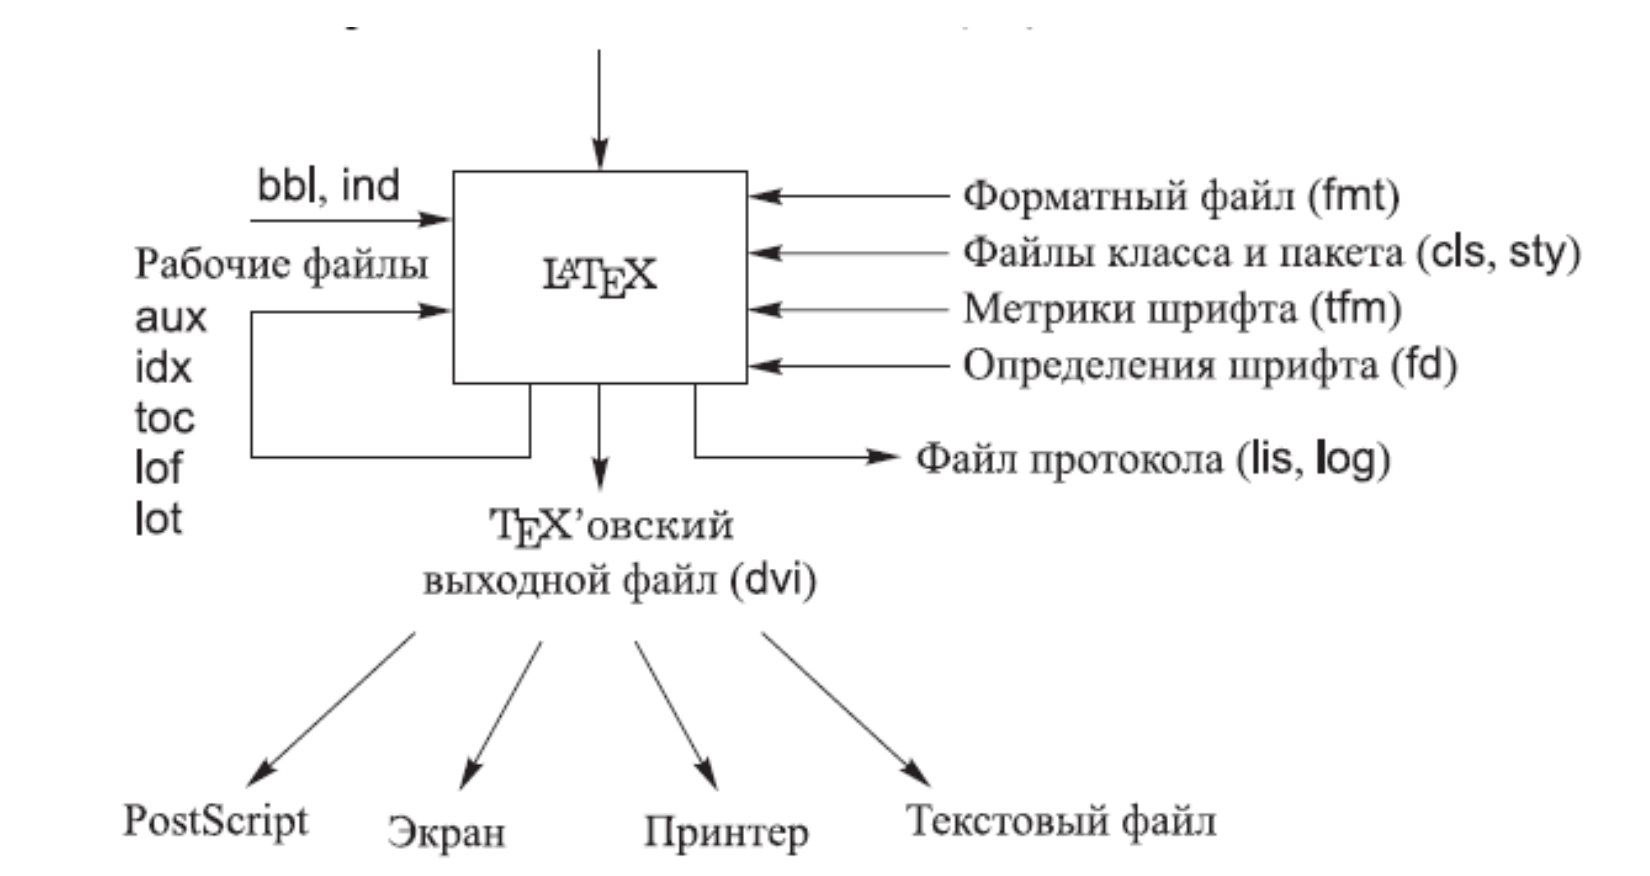
\includegraphics[scale=0.4]{img-1}

\section{Особенности набора текста в LATEX.}

\textbf{Комментарии.} Всё что следует за знаком «\%» является комментарием. Большие закомментированные сегменты мешают работать с основным тек- стом, и поэтому их следует исключать из рабочего файла. Но при желании можно воспользоваться окружением comment из пакета verbatim.

\textbf{Pазделение слов.} Пробельные символы используются в LATEX для разде- ления слов. Пробелы в начале строки игнорируются. Символ перевода строки так же воспринимается как пробел. Если в конце строки сразу за последним словом вставить знак комментария, то разделения слов не происходит. Ино- гда этот приём может оказаться полезным.

\textbf{Разделение абзацев.} Для того чтобы начать следующий абзац необхо- димо оставить пустую строку. Любое число пустых строк между абзацами эквивалентно одной.

\chapter{Практическая часть.}
\section{Задание №1}
В процессе выполнения серии команд в дириктории  появились файлы с расширениями .dvi ; 
.ps ; .log ; .pdf ; .aux

А при выполнение команды pdflatex, в директиве появились только .pdf ; .log ; .aux 
\section{Задание №2}

(...) 

\section{Задание №3}
В данном задание был реализован библиографический список, при помощи дополнительного пакета BiBTeX.




\end{document}
